\documentclass[12pt,oneside,a4paper]{article}
\usepackage[utf8]{inputenc}
\usepackage{tikz}
\usetikzlibrary{shapes,arrows}

\tikzstyle{line} = [draw, -latex']
\tikzset{%
  do path picture/.style={%
    path picture={%
      \pgfpointdiff{\pgfpointanchor{path picture bounding box}{south west}}%
        {\pgfpointanchor{path picture bounding box}{north east}}%
      \pgfgetlastxy\x\y%
      \tikzset{x=\x/2,y=\y/2}%
      #1
    }
  },
  cross/.style={do path picture={    
    \draw [line cap=round] (-1,-1) -- (1,1) (-1,1) -- (1,-1);
  }},
  dot/.style={do path picture={    
    \draw [fill]  circle [radius=1]; 
  }}
}
\begin{document}
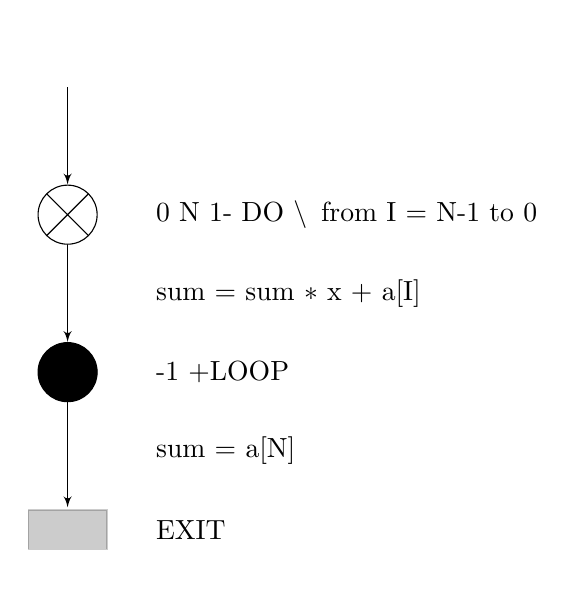
\begin{tikzpicture}[minimum size=0.75cm]
	\node at (1,7) (start) {\,};
	\node [circle, draw, cross]    at (1, 5) (cross) {};
	\node [right, align=left] at (2,5) {0 N 1- DO \textbackslash  \, from I = N-1 to 0} ;
	\node [right, align=left] at (2,4) {sum = sum $*$ x + a[I]} ;
	\node [circle, draw, dot]      at (1, 3) (dot)  {};
	\node [right, align=left] at (2,3) {-1 +LOOP} ;
	\node [right, align=left] at (2,2) {sum = a[N]} ;
	\draw [fill, opacity=0.2] (.5,1.25) rectangle (1.5,.75) {};
	\node at (1,0.90) (ext) {};
	\node [right, align=left] at (2,1) {EXIT} ;
	\path [line]  (cross) -- (dot);
	\path [line]  (dot) -- (ext);
	\path [line]  (start) -- (cross);
\end{tikzpicture}
\end{document}
